

\chapter{Flex Cloud}


StochSS 1.6 introduces Flex Cloud, an abstraction which allows you to run StochSS jobs on any machine, physical or virtual, provided it is running Ubuntu 12.04 with the required software dependencies installed. %Flex Cloud is a feature that should only be used by people familiar with the Linux operating systems, as it requires some detailed systems knowledge to set up.

\section{Setting Up Flex Cloud Compute Machines}

\subsection{Preparing the Flex Cloud compute nodes}
\begin{itemize}
\item Configure one or more machines running Ubuntu 12.04 (Precise). %It is recommended that these computers be dedicated solely to Flex Cloud, as to reduce the chance of interference between StochSS and other programs.
\item Please make sure the machines have their own IP address and are accessible with just a username and a passwordless SSH keypair. If necessary, generate SSH keypairs for the machines. You will need to upload the SSH private key to the StochSS user interface to access the machines.
\item Configure the firewall on the machines to allow connections on the following ports: 22, 5672, 6379, 11211, 55672, 80, 443, 3306. These are used for various services used by StochSS. If the machines are instances running on a public or private cloud, you may need to enable the ports by modifying the associated cloud security group. 
\item Install the software prerequisites on the machines by using the command line utility \emph{make\_flex\_vms.py}  which can be found in the StochSS Github repository in the directory \emph{release-tools/flex-cloud}. You can either specify the username, IP address, and SSH keys of the machines in a machine config file (an example one is included in the same directory for reference) or you can specify the machines on the command line. The script \emph{make\_flex\_vms.py} will also verify that the necessary network ports are open and working. Please see \emph{make\_flex\_vms.py -h} for further information.
\end{itemize}

\subsection{Configuring the compute nodes in StochSS}

\begin{itemize}
\item Click \textbf{Cloud Computing} to navigate to the main \textbf{Cloud Computing} page.
\item You have the option of selecting \textbf{Amazon AWS Cloud} or \textbf{Flex Cloud}. Select \textbf{Flex Cloud}. It will redirect you to \textbf{Flex Cloud Credentials} page. 

(Note: You cannot set up both Amazon AWS Cloud or Flex Cloud at the same time. If one cloud computing infrastructure has been set up, the link for the other infrastructure will be disabled on this page.)

%\begin{figure}[!ht]
%\centering
%\includegraphics[scale=0.45]{T7/T7_fig_flex_cloud_credentials_page.png}
%\caption{Flex Cloud Credentials page}
%\label{fig:2}
%\end{figure}

\item Click \textbf{Choose Files} to upload the SSH private keys (see Figure \ref{fig:2}).

\begin{figure}[!ht]
\centering
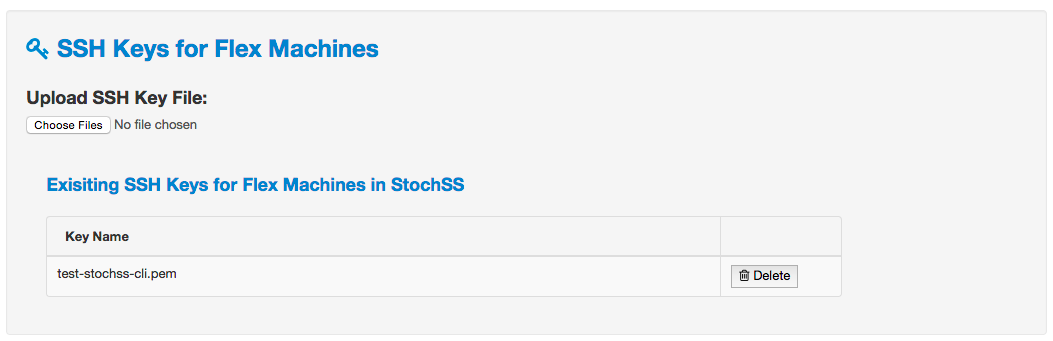
\includegraphics[scale=0.45]{T7/T7_fig_flex_uploaded_ssh_keys.png}
\caption{Uploaded SSH keys for Flex Machines -- Flex Cloud Credentials page}
\label{fig:2}
\end{figure}

\item Next, in the first row of the \textbf{Flex Cloud Machine Info} table, type the IP address and username, and select the appropriate key pair for the compute node that should act as the queue head. The Flex Queue Head will act as a coordinate for StochSS jobs, as well as store all output for jobs run in the cloud. This machine should be fairly robust; for EC2 instances a c3.large would be appropriate.
\item Click \textbf{+} to add more compute nodes. %For each of them, type the IP address, username, and enter the key info as above.
\item Click \textbf{Deploy} to start the Flex Cloud service.
\item The compute nodes may take a few minutes to launch. Refresh the page occasionally and wait until all nodes enter the \emph{Running} state as shown in the \textbf{Flex Cloud Machine Info} table.

\item Once Flex Cloud has been successfully configured, StochSS will run jobs in Flex Cloud when you click \textbf{Run via Cloud} as long as Flex Cloud has been successfully configured and the Flex Queue Head node is up and running.

\item To stop Flex Cloud, click \textbf{Stop} on the Flex Cloud configuration page. (Note: \textbf{Stop} does not terminate/shut-down/reboot machines).

\warning{\newline Any data that is not downloaded from the Flex Cloud will be inaccessible while the Flex Cloud is turned off. Reconfiguring the queue head or keys without downloading job results can lead to data loss.\newline}

\end{itemize}

